\documentclass{standalone}
\usepackage{tikz}
\usetikzlibrary{patterns, positioning}


\begin{document}
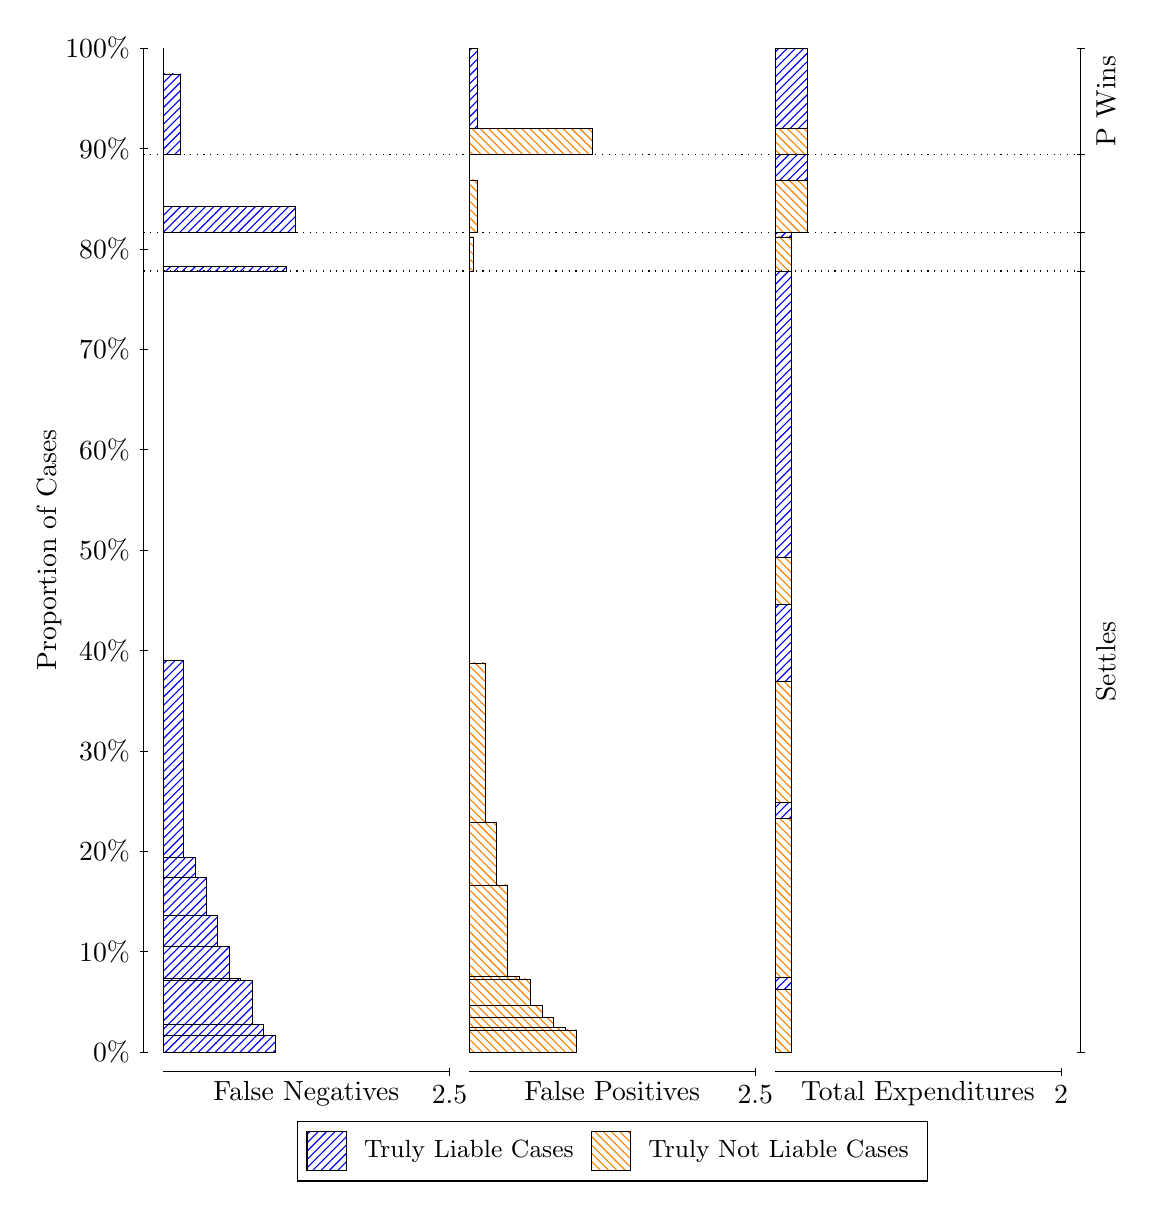
\begin{tikzpicture}
\draw[black, very thin] (1.5,1.75) -- (1.5,14.5);
\node[rotate=90, text=black, anchor=center] at (0.3, 8.125) {Proportion of Cases};
\draw[black, very thin] (1.45,1.75) -- (1.55,1.75);
\node[text=black, anchor=east] at (1.45, 1.75) {0\%};
\draw[black, very thin] (1.45,3.025) -- (1.55,3.025);
\node[text=black, anchor=east] at (1.45, 3.025) {10\%};
\draw[black, very thin] (1.45,4.3) -- (1.55,4.3);
\node[text=black, anchor=east] at (1.45, 4.3) {20\%};
\draw[black, very thin] (1.45,5.575) -- (1.55,5.575);
\node[text=black, anchor=east] at (1.45, 5.575) {30\%};
\draw[black, very thin] (1.45,6.85) -- (1.55,6.85);
\node[text=black, anchor=east] at (1.45, 6.85) {40\%};
\draw[black, very thin] (1.45,8.125) -- (1.55,8.125);
\node[text=black, anchor=east] at (1.45, 8.125) {50\%};
\draw[black, very thin] (1.45,9.4) -- (1.55,9.4);
\node[text=black, anchor=east] at (1.45, 9.4) {60\%};
\draw[black, very thin] (1.45,10.675) -- (1.55,10.675);
\node[text=black, anchor=east] at (1.45, 10.675) {70\%};
\draw[black, very thin] (1.45,11.95) -- (1.55,11.95);
\node[text=black, anchor=east] at (1.45, 11.95) {80\%};
\draw[black, very thin] (1.45,13.225) -- (1.55,13.225);
\node[text=black, anchor=east] at (1.45, 13.225) {90\%};
\draw[black, very thin] (1.45,14.5) -- (1.55,14.5);
\node[text=black, anchor=east] at (1.45, 14.5) {100\%};

\draw[black, very thin] (13.4,1.75) -- (13.4,14.5);
\draw[black, very thin] (13.35,1.75) -- (13.45,1.75);
\node[anchor=west] at (13.35, 1.75) {};
\draw[black, very thin] (13.35,11.668) -- (13.45,11.668);
\node[anchor=west] at (13.35, 11.668) {};
\draw[black, very thin] (13.35,12.156) -- (13.45,12.156);
\node[anchor=west] at (13.35, 12.156) {};
\draw[black, very thin] (13.35,13.153) -- (13.45,13.153);
\node[anchor=west] at (13.35, 13.153) {};
\draw[black, very thin] (13.35,14.5) -- (13.45,14.5);
\node[anchor=west] at (13.35, 14.5) {};

\draw[black, very thin, pattern color=blue, pattern=north east lines] (1.75,1.75) rectangle (3.167,1.957);
\draw[black, very thin, pattern color=blue, pattern=north east lines] (1.75,1.957) rectangle (3.0217,2.1019);
\draw[black, very thin, pattern color=blue, pattern=north east lines] (1.75,2.1019) rectangle (2.8763,2.6601);
\draw[black, very thin, pattern color=blue, pattern=north east lines] (1.75,2.6601) rectangle (2.731,2.683);
\draw[black, very thin, pattern color=blue, pattern=north east lines] (1.75,2.683) rectangle (2.5857,3.0871);
\draw[black, very thin, pattern color=blue, pattern=north east lines] (1.75,3.0871) rectangle (2.4403,3.483);
\draw[black, very thin, pattern color=blue, pattern=north east lines] (1.75,3.483) rectangle (2.295,3.9651);
\draw[black, very thin, pattern color=blue, pattern=north east lines] (1.75,3.9651) rectangle (2.1497,4.2205);
\draw[black, very thin, pattern color=blue, pattern=north east lines] (1.75,4.2205) rectangle (2.0043,6.7256);
\draw[black, very thin, pattern color=orange, pattern=north west lines] (1.75,6.7256) rectangle (1.75,11.668);
\draw[black, very thin, pattern color=blue, pattern=north east lines] (1.75,11.668) rectangle (3.3123,11.722);
\draw[black, very thin, pattern color=orange, pattern=north west lines] (1.75,11.722) rectangle (1.75,12.156);
\draw[black, very thin, pattern color=blue, pattern=north east lines] (1.75,12.156) rectangle (3.4213,12.484);
\draw[black, very thin, pattern color=orange, pattern=north west lines] (1.75,12.484) rectangle (1.75,13.153);
\draw[black, very thin, pattern color=blue, pattern=north east lines] (1.75,13.153) rectangle (1.968,14.171);
\draw[black, very thin, pattern color=orange, pattern=north west lines] (1.75,14.171) rectangle (1.75,14.5);
\draw[black, very thin, pattern color=orange, pattern=north west lines] (5.6333,1.75) rectangle (6.9958,2.0315);
\draw[black, very thin, pattern color=orange, pattern=north west lines] (5.6333,2.0315) rectangle (6.8505,2.0591);
\draw[black, very thin, pattern color=orange, pattern=north west lines] (5.6333,2.0591) rectangle (6.7052,2.1933);
\draw[black, very thin, pattern color=orange, pattern=north west lines] (5.6333,2.1933) rectangle (6.5598,2.3426);
\draw[black, very thin, pattern color=orange, pattern=north west lines] (5.6333,2.3426) rectangle (6.4145,2.6774);
\draw[black, very thin, pattern color=orange, pattern=north west lines] (5.6333,2.6774) rectangle (6.2692,2.7119);
\draw[black, very thin, pattern color=orange, pattern=north west lines] (5.6333,2.7119) rectangle (6.1238,3.8712);
\draw[black, very thin, pattern color=orange, pattern=north west lines] (5.6333,3.8712) rectangle (5.9785,4.6703);
\draw[black, very thin, pattern color=orange, pattern=north west lines] (5.6333,4.6703) rectangle (5.8332,6.6928);
\draw[black, very thin, pattern color=blue, pattern=north east lines] (5.6333,6.6928) rectangle (5.6333,11.668);
\draw[black, very thin, pattern color=orange, pattern=north west lines] (5.6333,11.668) rectangle (5.6878,12.102);
\draw[black, very thin, pattern color=blue, pattern=north east lines] (5.6333,12.102) rectangle (5.6333,12.156);
\draw[black, very thin, pattern color=orange, pattern=north west lines] (5.6333,12.156) rectangle (5.7423,12.826);
\draw[black, very thin, pattern color=blue, pattern=north east lines] (5.6333,12.826) rectangle (5.6333,13.153);
\draw[black, very thin, pattern color=orange, pattern=north west lines] (5.6333,13.153) rectangle (7.1957,13.482);
\draw[black, very thin, pattern color=blue, pattern=north east lines] (5.6333,13.482) rectangle (5.7423,14.5);
\draw[black, very thin, pattern color=orange, pattern=north west lines] (9.5167,1.75) rectangle (9.721,2.5491);
\draw[black, very thin, pattern color=blue, pattern=north east lines] (9.5167,2.5491) rectangle (9.721,2.6941);
\draw[black, very thin, pattern color=orange, pattern=north west lines] (9.5167,2.6941) rectangle (9.721,4.7165);
\draw[black, very thin, pattern color=blue, pattern=north east lines] (9.5167,4.7165) rectangle (9.721,4.9235);
\draw[black, very thin, pattern color=orange, pattern=north west lines] (9.5167,4.9235) rectangle (9.721,6.4522);
\draw[black, very thin, pattern color=blue, pattern=north east lines] (9.5167,6.4522) rectangle (9.721,7.4373);
\draw[black, very thin, pattern color=orange, pattern=north west lines] (9.5167,7.4373) rectangle (9.721,8.0299);
\draw[black, very thin, pattern color=blue, pattern=north east lines] (9.5167,8.0299) rectangle (9.721,11.668);
\draw[black, very thin, pattern color=orange, pattern=north west lines] (9.5167,11.668) rectangle (9.721,12.102);
\draw[black, very thin, pattern color=blue, pattern=north east lines] (9.5167,12.102) rectangle (9.721,12.156);
\draw[black, very thin, pattern color=orange, pattern=north west lines] (9.5167,12.156) rectangle (9.9254,12.826);
\draw[black, very thin, pattern color=blue, pattern=north east lines] (9.5167,12.826) rectangle (9.9254,13.153);
\draw[black, very thin, pattern color=orange, pattern=north west lines] (9.5167,13.153) rectangle (9.9254,13.482);
\draw[black, very thin, pattern color=blue, pattern=north east lines] (9.5167,13.482) rectangle (9.9254,14.5);
\draw[black, dotted] (1.5,11.668) -- (13.4,11.668);
\draw[black, dotted] (1.5,12.156) -- (13.4,12.156);
\draw[black, dotted] (1.5,13.153) -- (13.4,13.153);
\draw[black, very thin] (1.75,1.5) -- (5.3833,1.5);
\node[text=black, anchor=north] at (3.5667, 1.5) {False Negatives};
\draw[black, very thin] (5.3833,1.45) -- (5.3833,1.55);
\node[text=black, anchor=north] at (5.3833, 1.45) {2.5};

\draw[black, very thin] (5.6333,1.5) -- (9.2667,1.5);
\node[text=black, anchor=north] at (7.45, 1.5) {False Positives};
\draw[black, very thin] (9.2667,1.45) -- (9.2667,1.55);
\node[text=black, anchor=north] at (9.2667, 1.45) {2.5};

\draw[black, very thin] (9.5167,1.5) -- (13.15,1.5);
\node[text=black, anchor=north] at (11.333, 1.5) {Total Expenditures};
\draw[black, very thin] (13.15,1.45) -- (13.15,1.55);
\node[text=black, anchor=north] at (13.15, 1.45) {2};

\node[text=black, centered, rotate=90] at (13.72, 6.7092) {Settles};


\node[text=black, centered, rotate=90] at (13.72, 13.827) {P Wins};

\draw (7.449999999999999,1.5) node[draw=none] (baseCoordinate) {};
\begin{scope}[align=center]
        \matrix[scale=0.5, draw=black, below=0.5cm of baseCoordinate, nodes={draw}, column sep=0.1cm]{
            \node[rectangle, draw, minimum width=0.5cm, minimum height=0.5cm, pattern color=blue, pattern=north east lines] {}; &
            \node[draw=none, font=\small, text=black] (B) {Truly Liable Cases}; &
            \node[rectangle, draw, minimum width=0.5cm, minimum height=0.5cm, pattern color=orange, pattern=north west lines] {}; &
            \node[draw=none, font=\small, text=black] (B) {Truly Not Liable Cases}; \\
            };
\end{scope}

\end{tikzpicture}
\end{document}